\documentclass[11pt,landscape,a4paper]{article}
%\usepackage[utf8]{inputenc}
%\usepackage[ngerman]{babel}
\usepackage[normalem]{ulem}
\usepackage{tikz}
\usetikzlibrary{shapes,positioning,arrows,fit,calc,graphs,graphs.standard}
\usepackage[nosf]{kpfonts}
\usepackage[t1]{sourcesanspro}
%\usepackage[lf]{MyriadPro}
%\usepackage[lf,minionint]{MinionPro}
\usepackage{multicol}
\usepackage{wrapfig}
\usepackage[top=0mm,bottom=1mm,left=0mm,right=1mm]{geometry}
\usepackage[framemethod=tikz]{mdframed}
\usepackage{microtype}
%\usepackage{physics}
\usepackage{tabularx}
\usepackage{hhline}
\usepackage{makecell}
\usepackage{mathtools}

\usepackage{listings}

\DeclarePairedDelimiter{\ceil}{\lceil}{\rceil}

\newcommand\codeblue[1]{\textcolor{blue}{\code{#1}}}

\usepackage{lastpage}
\usepackage{datetime}
\yyyymmdddate
\renewcommand{\dateseparator}{-}
\let\bar\overline

\definecolor{myblue}{cmyk}{1,.72,0,.38}

\def\firstcircle{(0,0) circle (1.5cm)}
\def\secondcircle{(0:2cm) circle (1.5cm)}

\colorlet{circle edge}{myblue}
\colorlet{circle area}{myblue!5}

\tikzset{filled/.style={fill=circle area, draw=circle edge, thick},
outline/.style={draw=circle edge, thick}}

\pgfdeclarelayer{background}
\pgfsetlayers{background,main}

%\everymath\expandafter{\the\everymath \color{myblue}}
%\everydisplay\expandafter{\the\everydisplay \color{myblue}}


\renewcommand{\baselinestretch}{.8}
\pagestyle{empty}

\global\mdfdefinestyle{header}{%
  linecolor=gray,linewidth=1pt,%
  leftmargin=0mm,rightmargin=0mm,skipbelow=0mm,skipabove=0mm,
}

\newcommand{\header}{
  \begin{mdframed}[style=header]
    \footnotesize
    \sffamily
    CS3243 Finals Cheatsheet v1.1 (\today)\\
    by~Julius Putra Tanu Setiaji,~page~\thepage~of~\pageref{LastPage}
  \end{mdframed}
}

\let\counterwithout\relax
\let\counterwithin\relax
\usepackage{chngcntr}

\usepackage{verbatim}

\usepackage{etoolbox}
\makeatletter
\preto{\@verbatim}{\topsep=0pt \partopsep=0pt }
\makeatother

\counterwithin*{equation}{section}
\counterwithin*{equation}{subsection}
\usepackage{enumitem}
\newlist{legal}{enumerate}{10}
\setlist[legal]{label*=\arabic*.,leftmargin=2.5mm}
\setlist[itemize]{leftmargin=3mm}
\setlist[enumerate]{leftmargin=3.5mm}
\setlist{nosep}
\usepackage{minted}

\def\code#1{\texttt{#1}}

\newenvironment{descitemize} % a mixture of description and itemize
{\begin{description}[leftmargin=*,before=\let\makelabel\descitemlabel]}
{\end{description}}

\newcommand{\descitemlabel}[1]{%
  \textbullet\ \textbf{#1}%
}
\makeatletter



\renewcommand{\section}{\@startsection{section}{1}{0mm}%
  {.2ex}%
  {.2ex}%x
{\color{myblue}\sffamily\small\bfseries}}
\renewcommand{\subsection}{\@startsection{subsection}{1}{0mm}%
  {.2ex}%
  {.2ex}%x
{\sffamily\bfseries}}
\renewcommand{\subsubsection}{\@startsection{subsubsection}{1}{0mm}%
  {.2ex}%
  {.2ex}%x
{\rmfamily\bfseries}}



\def\multi@column@out{%
  \ifnum\outputpenalty <-\@M
    \speci@ls \else
  \ifvoid\colbreak@box\else
    \mult@info\@ne{Re-adding forced
    break(s) for splitting}%
    \setbox\@cclv\vbox{%
      \unvbox\colbreak@box
    \penalty-\@Mv\unvbox\@cclv}%
  \fi
  \splittopskip\topskip
  \splitmaxdepth\maxdepth
  \dimen@\@colroom
  \divide\skip\footins\col@number
  \ifvoid\footins \else
    \leave@mult@footins
  \fi
  \let\ifshr@kingsaved\ifshr@king
    \ifvbox \@kludgeins
      \advance \dimen@ -\ht\@kludgeins
      \ifdim \wd\@kludgeins>\z@
        \shr@nkingtrue
      \fi
    \fi
    \process@cols\mult@gfirstbox{%
      %%%%% START CHANGE
      \ifnum\count@=\numexpr\mult@rightbox+2\relax
        \setbox\count@\vsplit\@cclv to \dimexpr \dimen@-1cm\relax
        \setbox\count@\vbox to \dimen@{\vbox to 1cm{\header}\unvbox\count@\vss}%
      \else
        \setbox\count@\vsplit\@cclv to \dimen@
      \fi
      %%%%% END CHANGE
      \set@keptmarks
      \setbox\count@
      \vbox to\dimen@
      {\unvbox\count@
        \remove@discardable@items
    \ifshr@nking\vfill\fi}%
    }%
    \setbox\mult@rightbox
    \vsplit\@cclv to\dimen@
    \set@keptmarks
    \setbox\mult@rightbox\vbox to\dimen@
    {\unvbox\mult@rightbox
      \remove@discardable@items
  \ifshr@nking\vfill\fi}%
    \let\ifshr@king\ifshr@kingsaved
  \ifvoid\@cclv \else
    \unvbox\@cclv
    \ifnum\outputpenalty=\@M
  \else
    \penalty\outputpenalty
  \fi
  \ifvoid\footins\else
    \PackageWarning{multicol}%
    {I moved some lines to
      the next page.\MessageBreak
      Footnotes on page
    \thepage\space might be wrong}%
  \fi
  \ifnum \c@tracingmulticols>\thr@@
\hrule\allowbreak \fi
  \fi
  \ifx\@empty\kept@firstmark
    \let\firstmark\kept@topmark
    \let\botmark\kept@topmark
  \else
    \let\firstmark\kept@firstmark
    \let\botmark\kept@botmark
  \fi
  \let\topmark\kept@topmark
  \mult@info\tw@
  {Use kept top mark:\MessageBreak
    \meaning\kept@topmark
    \MessageBreak
    Use kept first mark:\MessageBreak
    \meaning\kept@firstmark
    \MessageBreak
    Use kept bot mark:\MessageBreak
    \meaning\kept@botmark
    \MessageBreak
    Produce first mark:\MessageBreak
    \meaning\firstmark
    \MessageBreak
    Produce bot mark:\MessageBreak
    \meaning\botmark
  \@gobbletwo}%
  \setbox\@cclv\vbox{\unvbox\partial@page
  \page@sofar}%
  \@makecol\@outputpage
  \global\let\kept@topmark\botmark
  \global\let\kept@firstmark\@empty
  \global\let\kept@botmark\@empty
  \mult@info\tw@
  {(Re)Init top mark:\MessageBreak
    \meaning\kept@topmark
  \@gobbletwo}%
  \global\@colroom\@colht
  \global \@mparbottom \z@
  \process@deferreds
\@whilesw\if@fcolmade\fi{\@outputpage
    \global\@colroom\@colht
  \process@deferreds}%
  \mult@info\@ne
  {Colroom:\MessageBreak
    \the\@colht\space
    after float space removed
  = \the\@colroom \@gobble}%
  \set@mult@vsize \global
  \fi}
  \global\let\tikz@ensure@dollar@catcode=\relax

  \def\mathcolor#1#{\@mathcolor{#1}}
  \def\@mathcolor#1#2#3{%
    \protect\leavevmode
    \begingroup
    \color#1{#2}#3%
    \endgroup
  }

  \makeatother
  \setlength{\parindent}{0pt}

  \setminted{tabsize=2, breaklines}
  % Remove belowskip of minted
  \setlength\partopsep{-\topsep}


  \newcolumntype{a}{>{\hsize=1.5\hsize}X}
  \newcolumntype{b}{>{\hsize=.25\hsize}X}

  \setlength\columnsep{1.5pt}
  \setlength\columnseprule{0.1pt}

\begin{document}
\setlength{\abovedisplayskip}{0pt}
\setlength{\belowdisplayskip}{0pt}


\tiny
\begin{multicols*}{4}
  \raggedcolumns
  \section{Introduction to AI}
  \subsection{Rational Agent}
  \begin{itemize}
    \item An \textbf{agent} is an entity that perceives its \textbf{env} through sensors \& acts through \textbf{actuators}
    \item An agent's \textbf{percept sequence} is complete history of everything the agent has ever perceived.
    \item What is rational depends on: (1) The performane measure that defines success, (2) The agent's prior knowledge of the env, (3) The actions that the agent can perform, (4) The agent's percept sequence to date.
    \item For each possible percept sequence, a \textbf{Rational Agent} should select an action that is expected to maximise its performance measure, given the evidence provided by the percept sequence and whatever built-in knowledge the agent has.
  \end{itemize}
  \subsection{Task Environment}
  \begin{itemize}
    \item \textbf{PEAS}: Performance, Environment, Actuators, Sencsors
    \item \textbf{Fully observable} vs \textbf{Partially observable}:: an agent's sensors give it access to the complete state of the env at each point in time \textbf{VS} if the sensors detect all aspects that are relevant to the choice of action
    \item \textbf{Single agent} vs \textbf{Multiagent}: whether there are any other agent in the environment, multiagent further divided into \textbf{competitive} and \textbf{cooperative} where \textbf{communication} and \textbf{randomised behaviour} are the typical rational behaviours respectively
    \item \textbf{Deterministic} vs \textbf{Stochastic}: if the next state of the env is completely determined by the current state and the action executed by the agent \textbf{VS} otherwise. (partially observable env may appear stochastic)
    \item \textbf{Episodic} vs \textbf{Sequential}: the choice of current action does not depend on prev actions \textbf{VS} otherwise
    \item \textbf{Static} vs \textbf{Dynamic}: if the environment is unchanged while an agent is deliberating \textbf{VS} otherwise
    \item \textbf{Discrete} vs \textbf{Continuous}: in terms of state of env, time, percepts and actions
  \end{itemize}
  \subsection{The Structure of Agents}
  \begin{itemize}
    \item An \textbf{agent program} (takes in current percept) implements the \textbf{agent function} (percept sequence): mapping from percept sequence to actions.
    \item \textbf{Table-Driven-Agent}: persists the percept sequence from the current percept, and looks up action from table.
    \item Drawback: Hube table to build and store (time and space), no autonomy (impossible to learn all correct table entries from experience), no guidance on filling in the correct tabel entries
  \end{itemize}
  \subsection{Agent Types, in increasing generality}
  \begin{itemize}
    \item \textbf{Simple Reflex Agent}: passive, only selects actions on the basis of the current percept (ignoring percept history). Updates state based on percept only
    \item The rest updates state based on percept, current state, most recent action and model of the world.
    \item \textbf{Model-based Reflex Agents}: passive, (to handle partial observability, need to build model of the world)
    \item \textbf{Goal-based Agent}: achieve goal (binary: achieve goal/not).
    \item \textbf{Utility-based Agent}: maximises utility function (measure of happiness: more than binary).
    \item \textbf{Learning Agent}: \textbf{Learning element} responsible for making improvements with feedback from the \textbf{critic}, \textbf{performance element} (what was agent) responsible for selecting external actions, \textbf{problem generator} responsible for suggesting actions (do suboptimal now to explore better actions in the long run).
  \end{itemize}

  \section{Solving Problems by Searching}
  \subsection{Problem Formulation}
  \textbf{Initial State}, \textbf{Actions} (set of actions possible given a particular state), \textbf{Transition Models} (description of each action), \textbf{Goal Test} (determines whether a state is a goal state), \textbf{Path Cost } (assigns a numeric cost to each path)

  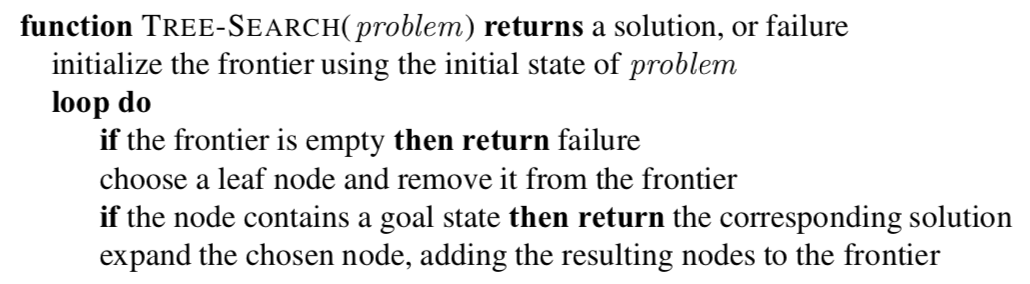
\includegraphics[width=\columnwidth]{tree-search}
  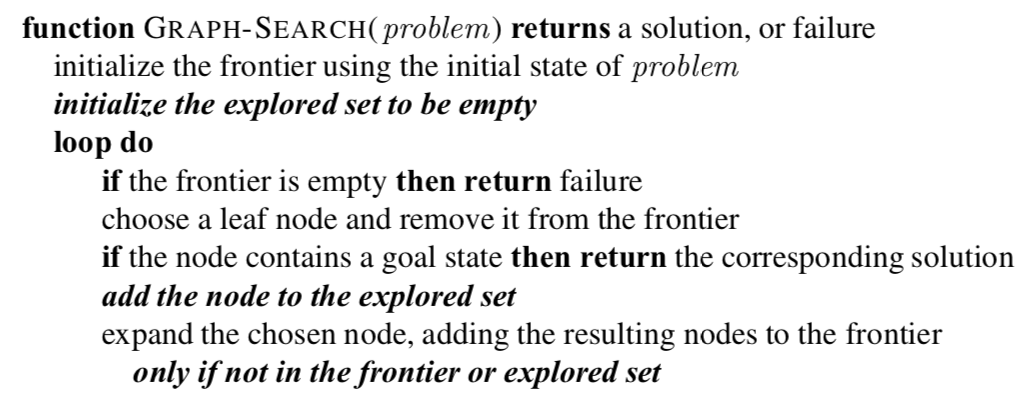
\includegraphics[width=\columnwidth]{graph-search}

  A \textbf{node} includes state, parent node, action, and path cost.
  \subsection{Evaluation criteria}
  \begin{itemize}
    \item \textbf{Completeness}: always find solution if one exists
    \item \textbf{Optimality}: finding a least-cost solution
    \item \textbf{Time complexity}: no of nodes generated
    \item \textbf{Space complexity}: max. no of nodes in memory
  \end{itemize}
  \subsection{Problem parameters}
  \begin{itemize}
    \item $b$: max. no of successors of any node
    \item $d$: depth of shallowest goal node
    \item $m$: max. depth of search tree
  \end{itemize}
  \textbf{Uninformed Search Strategies}

  \begin{tabular}{l|l|l|l|l|l}
    \textbf{Property} & \textbf{BFS} & \textbf{UCS}                                             & \textbf{DFS} & \textbf{DLS} & \textbf{IDS} \\ \hline
    \textbf{Complete} & Yes*         & Yes**                                                    & No***        & No           & Yes*         \\
    \textbf{Optimal}  & No*          & Yes                                                      & No           & No           & No*          \\
    \textbf{Time}     & $O(b^dt)$    & $O(b^{1+\left\lfloor\frac{C^*}{\epsilon}\right\rfloor})$ & $O(b^m)$     & $O(b^l)$     & $O(b^d)$     \\
    \textbf{Space}    & $O(b^d)$     & $O(b^{1+\left\lfloor\frac{C^*}{\epsilon}\right\rfloor})$ & $O(bm)$      & $O(bl)$      & $O(bd)$      \\
  \end{tabular}

  *: BFS, IDS -- complete if $b$ is finite, optimal if step costs are identical

  **: UCS is complete if $b$ is finite and step cost $\geq\epsilon$

  ***: DFS is complete only on infinite depth graphs

  $C^*$ is the optimal cost

  \subsection{Breadth-First Search (BFS)}
  Expand shallowest unexpanded node, frontier is FIFO
  \subsection{Uniform-Cost Search (UCS)}
  Expand least-path-cost unexpanded node, frontier is PQ by path cost. Equivalent to BFS if all step costs are equal
  \subsection{Depth-First Search (DFS)}
  \begin{itemize}
    \item Expand deepest unexpanded node, frontier is LIFO.
    \item \textbf{Backtraking Search}, space can be $O(m)$ if successor is expanded one at a time (partially expanded node remembers which successor to generate next)
  \end{itemize}
  \subsection{Depth-Limited Search (DLS)}
  Run DFS with depth limit $l$, to solve the infinite-path problem
  \subsection{Iterative Deepening Search (IDS)}
  \begin{itemize}
    \item  Perform DLS with increasing depth limit.
    \item Preferred if search space is large and depth of solution is not known
  \end{itemize}
  \textbf{Informed (Heuristic Search Strategies)}

  Use an \textbf{evaluation function} $f(n)$ for each node $n$
  \subsection{Greedy best-first search}
  \begin{itemize}
    \item $f(n) = h(n) = $ estimated cost of cheapest path from $n$ to goal
    \item Expands nodes that appear to be closest to the goal
    \item \textbf{Complete} if $b$ is finite, \textbf{Non-optimal}, \textbf{Time} $O(b^m)$, \textbf{Space} $O(b^m)$
  \end{itemize}
  \subsection{A* Search}
  \begin{itemize}
    \item $f(n) = g(n) + h(n)$ where $g(n) = $ path cost from start node to node $n$
    \item Avoids expanding paths that are already expensive
    \item \textbf{Admissible Heuristic} never overestimates the cost to reach the goal: $\forall n, h(n) \leq h^*(n)$ where $h^*(n) = $ true cost
    \item \textbf{Consistent Heuristic}: triangle inequality -- $h(n) \leq c(n, n') + h(n')$
    \item Every consistent heuristic is also admissible.
    \item Theorem: If $h(n)$ is admissible, then A* tree-search is optimal
    \item Theorem: If $h(n)$ is consistent, then A* graph-search is optimal (from lemma consistent heuristic always follow optimal path)
    \item \textbf{Complete} if there is a finite no of nodes with $f(n) \leq f(G)$, \textbf{Optimal}, \textbf{Time} $O^{h^*(s_0) - h(s_0)}$ where $h^*(s_0)$ is the actual cost of getting from root to goal, \textbf{Space} $O(b^m)$
    \item \textbf{Dominant heuristic}: if $\forall n, h_2(n) \geq h_1(n)$ then $h_2$ \textbf{dominates} $h_1$
    \item More dominant heuristics incur lower search cost
  \end{itemize}

  \section{Beyond Classical Search}
  \begin{itemize}
    \item Path to goal is irrelevant, the goal state itself is the solution.
    \item Advantages: (1) use very little/constant memory, (2) can find reasonable solns in large/infinite continuous state spaces
    \item Useful for \textbf{pure optimization problems}: objective is to find the best state according to an \textbf{objective function}
  \end{itemize}
  \subsection{Hill-climbing Search (aka Greedy Local Search)}
  \begin{itemize}
    \item Continually moves in the direction of icnreasing value, terminate when reaching a "peak"
    \item Possible to get stuck in local maxima, only use if OK with approximate solutions.
  \end{itemize}

  \section{Adversarial Search}
  \begin{itemize}
    \item 2 players, zero-sum game
    \item \textbf{Game formulation}:
          \begin{itemize}
            \item $S_0$: The \textbf{initial state}
            \item PLAYER(s): which player has the move in a state
            \item ACTIONS(s): returns the set of legal moves in a state.
            \item RESULT(s, a): The \textbf{transition model}, defines the result of a move
            \item TERMINAL-TEST(s): A \textbf{terminal test}, true when game is over
            \item UTILITY(s, p): A \textbf{utility function)}, defines final numeric value for a game that ends in terminal state $s$ for a player $p$
          \end{itemize}
  \end{itemize}
  \subsection{Optimal Decisions in Games}
  \begin{itemize}
    \item \textbf{Winning} strategy for one player if for any strategy played by the other player, the game ended with the former as the winner. Similar for \textbf{non-losing} strategy.
    \item \textbf{Nash Equilibrium} -- when players know the strategies of all opponents, no one wants to change their strategy.
    \item \textbf{Subgame Perfect Nash Eq} -- every subgame is a \textbf{Nash Eq}
  \end{itemize}
  \subsection{Minimax}
  \begin{itemize}
    \item Optimal strategy can be determined from \textbf{minimax value} of each node: utility (for MAX) of being in the state, assuming both players play optimally from there to end of the game.
    \item Minimax returns a subperfect Nash equilibrium
    \item \textbf{Complete} (with finite game tree), \textbf{Optimal}, \textbf{Time} $O(b^m)$, \textbf{Space} $O(bm)$
  \end{itemize}
  \subsection{$\alpha-\beta$ Pruning}
  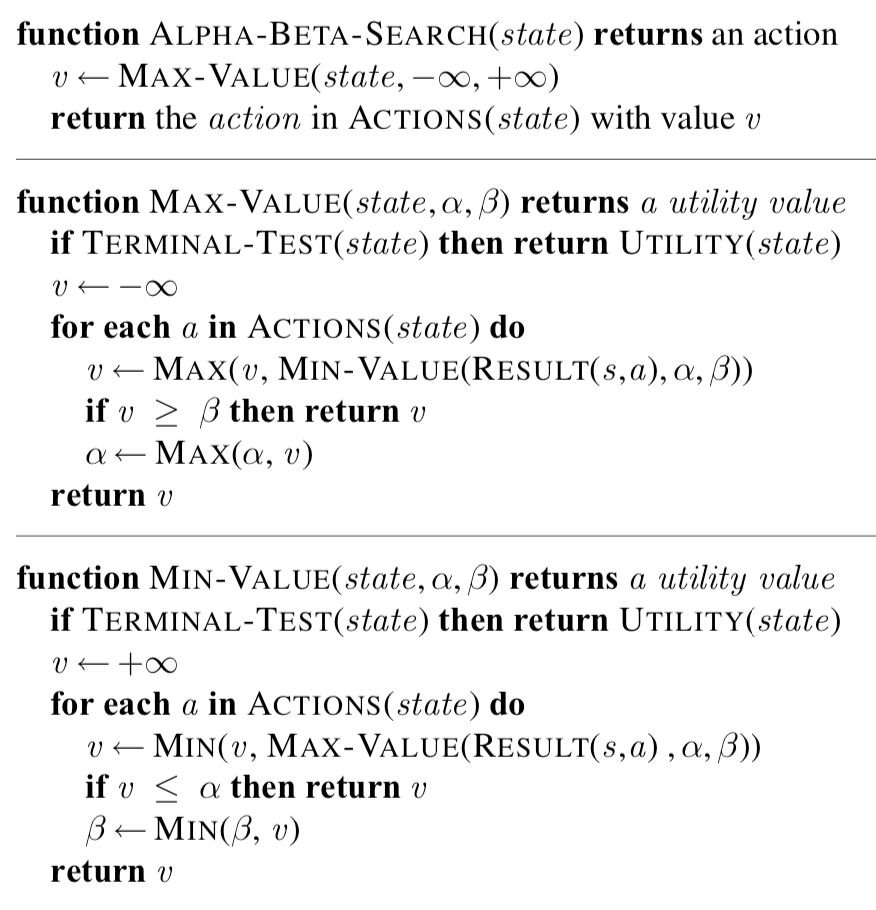
\includegraphics[width=0.8\columnwidth]{alpha-beta}
  \begin{itemize}
    \item MAX node n: $\alpha(n) = $ highest observed value found on path from n, initially $-\infty$
    \item MIN node n: $\beta = $ lowest observed value found on path from n, initially $+\infty$
    \item If a MIN node has value $v \leq \alpha(n)$, can prune
    \item If a MAX node has value $v \geq \beta(n)$, can prune
  \end{itemize}

  \subsection{Imperfect Real-time Decisions}
  \begin{itemize}
    \item Although very large search space in typical games is pruned by $\alpha-\beta$ pruning, minimax still has to search all the way to the terminal states.
    \item Replace utility function with heuristic \textbf{evaluation function} that estimates the position's utility, and replace the terminal test with a \textbf{cutoff test} that decides when to apply EVAL.
  \end{itemize}
  \subsection{Evaluation Functions}
  \begin{itemize}
    \item A mapping from game states to real values.
    \item Should be cheap to compute; for non-terminal states, must be strongly correlated with actual chances of winning
    \item Modern eval function: weighted sum of position features
    \item Need not return actual expected values, just maintain relative order of states, typically from statistically probabilities
  \end{itemize}
  \subsection{Cutting off Search}
  Stop after a certain depth, can be combined with iterative deepening

  \section{Constraint Satisfaction Problems}
  Consists of 3 components:
  \begin{itemize}
    \item $X$ is a set of variables, $\{X_1, ..., X_n\}$
    \item $D$ is a set of domains, $\{D_1, ..., D_n\}$, one for each variable
    \item $C$ is a set of constraints that specify allowable combinations of values
  \end{itemize}
  \subsection{Terminologies}
  \begin{itemize}
    \item \textbf{Consistent} assignment = does not vilate any constraints
    \item \textbf{Complete} assignment = every variable is assigned
    \item Goal: find a consistent and complete assignment
    \item \textbf{Binary constraint} relates 2 variables
    \item \textbf{Global constraint} involve an arbitrary number of variables
    \item Every finite-domain constraint can be reduced to a set of binary constraints if enough auxiliary variables are introduced.
    \item \textbf{Constraint graph}: nodes are variables, links are constraints
  \end{itemize}
  \subsection{Variants}
  \begin{itemize}
    \item Domain can be \textbf{discrete} (both \textbf{finite} and \textbf{infinite}) or \textbf{continuous}
    \item For discrete, infinite domains, a \textbf{constraint language} must be used without enumeration
  \end{itemize}
  \subsection{Constraint propagation: Inference in CSP}
  Try to infer illegal values for variables by performing constraint propagation

  For unary constraints, node consistency; For binary constraints, arc consistency

  \textbf{Arc Consistency} = a variable $X_i$ in CSP is arc-consistent with another variable $X_j$ if for every value in the current domain $D_i$ there is some value in the domain $D_j$ that satisfies the binary constraint on the arc $(X_i,X_j)$. A network is arc-consistent if every variable is arc-consistent with every other variable.

  \textbf{Time} $O(n^2d^3)$ where $n$ is number of vars, $d$ is max domain size

  \textbf{$K$-consistency} = if, for any set of $k-1$ vars and for any consistent assignment to those variables, a consistent value can always be assigned to any $k$-th var (arc-consistency is 2-consistency)

  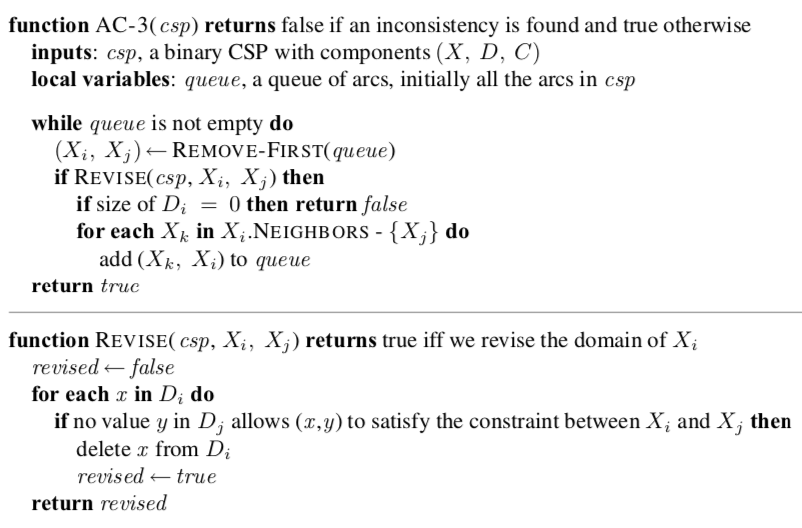
\includegraphics[width=\columnwidth]{ac-3}

  \subsection{Backtracking Search for CSPs}
  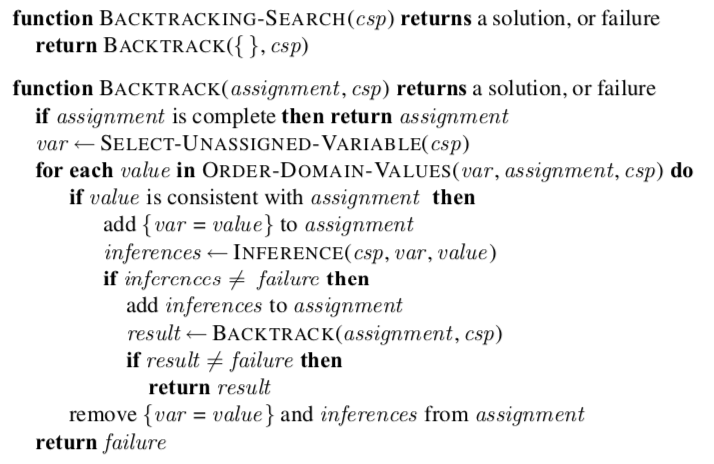
\includegraphics[width=\columnwidth]{backtrack}
  \begin{itemize}
    \item Better an just doing search, because CSPs are \textbf{commutative}
    \item DFS that chooses values for one variable at a time, and backtracks when a var has no legal values left to assign.
    \item For SELECT-UNASSIGNED-VARIABLE: use \textbf{Most Constrained Variable} choose the var with fewest legal values (Minimum Remaining Values (MRV) heuristic)
    \item Once a variable is selected, to decide the order to examine its values, use \textbf{Least Constraining Value} heuristic: prefer value that rules out the fewest choices for the neighbouring variables in the constraint graph
  \end{itemize}
  \subsection{Local Search for CSPs}
  \begin{itemize}
    \item Similar to hill-climbing, but instead with complete states, allow states that violate constraints, then reassign variable values
    \item In choosing a new value for a variable, herustic: select the value that results in the minimum number of conflicts with other variables
  \end{itemize}
  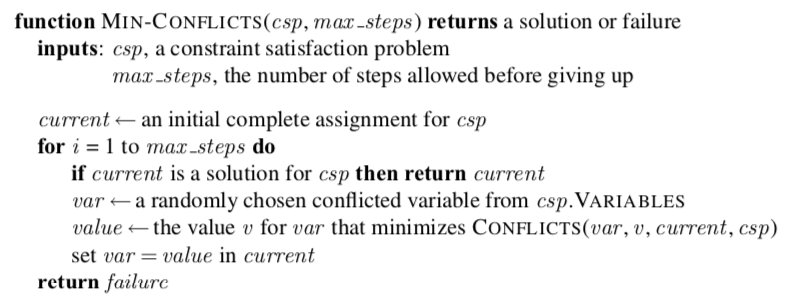
\includegraphics[width=\columnwidth]{min-conflict}
  \subsection{The structure of problems}
  \begin{itemize}
    \item Theorem: if CSP constraint graph (with binary constraints) is a \textbf{tree}, then we can compute a satisfying assignment (or determine one does not exist) in $O(nd^2)$ time (no need to backtrack)
    \item Proof: Pick any variable to be the root of tree, and choose an ordering of vars such that each var appears after its parent in the tree (Toposort: $O(n)$, each of which must compare up to $d$ possible domain values for the two variables)
  \end{itemize}

  \section{Logical Agents}
  \subsection{Knowledge-based Agents}
  \begin{itemize}
    \item Inference Engine (domain-independent algorithms)
    \item \textbf{Knowledge base} = set of sentences in a formal language (domain-specific content)
    \item Declarative approach to building an agent: \textsc{Tell} it what it needs to know, then it can \textsc{Ask} itself what todo according to the KB
  \end{itemize}
  \subsection{Logic}
  \begin{itemize}
    \item \textbf{Logic} = formal language for KR, infer conclusions
    \item \textbf{Syntax} = defines the sentences in the language
    \item Semantics = define the ``meaning'' of sentences (truth of a sentence in a world)
  \end{itemize}
  \subsection{Entailment}
  \begin{itemize}
    \item \textbf{Modeling}: $m$ models $\alpha$ if $\alpha$ is true under $m$.
    \item Let $M(\alpha)$ be the set of all models for $\alpha$
    \item \textbf{Entailment} means that one thing follows logically from another sentence: $\alpha \models \beta \iff M(\alpha) \subseteq M(\beta)$
    \item Properties of inference algorithms:
          \begin{itemize}
            \item \textbf{Sound} or \textbf{Truth-preserving} -- derives only entailed sentences
            \item \textbf{Completeness} -- it can derive any sentence that is entailed
          \end{itemize}
  \end{itemize}

  \section{Propositional Logic}
  \subsection{Syntax}
  \begin{itemize}
    \item Atomic sentences consisting of a single proposition symbol
    \item Complex sentences constructed from simpler sentences using parantheses and \textbf{logical connectives}: $\lnot$ (not), $\land$ (and), $\lor$ (or), $\implies$~(implies), $\iff$~(iff/biconditional)
  \end{itemize}
  \subsection{Semantics}
  A \textbf{truth assignment} to every proposition symbol.
  \subsection{Validity and Satisfiability}
  \begin{itemize}
    \item A sentence is \textbf{valid} if it is true in \textbf{all} models (e.g. $A\Rightarrow A$, $A\lor\lnot A$)
    \item A sentence is \textbf{satisfiable} if it is true in \textbf{some} model (e.g. $A\lor B$)
    \item A sentence is \textbf{unsatisfiable} if it is true in \textbf{no} model (e.g. $A\land\lnot A$)
  \end{itemize}
  \subsection{Inference}
  \begin{itemize}
    \item By \textbf{Truth-Table Enumeration}, DFS is sound and complete, time $O(2^n)$, space $O(n)$
    \item \textbf{Deduction Thm}:\\
          $KB \models \alpha \iff (KB \implies \alpha)$ is valid $\iff (KB \land\lnot\alpha)$ is unsatisfiable
  \end{itemize}
  \subsection{Inference Rules}
  \begin{itemize}
    \item \textbf{Modus Ponens}: $a \land (a \implies b) \models b$
    \item \textbf{And-Elimination}: $a \land b \models a$
    \item Logical equivalences:
  \end{itemize}
  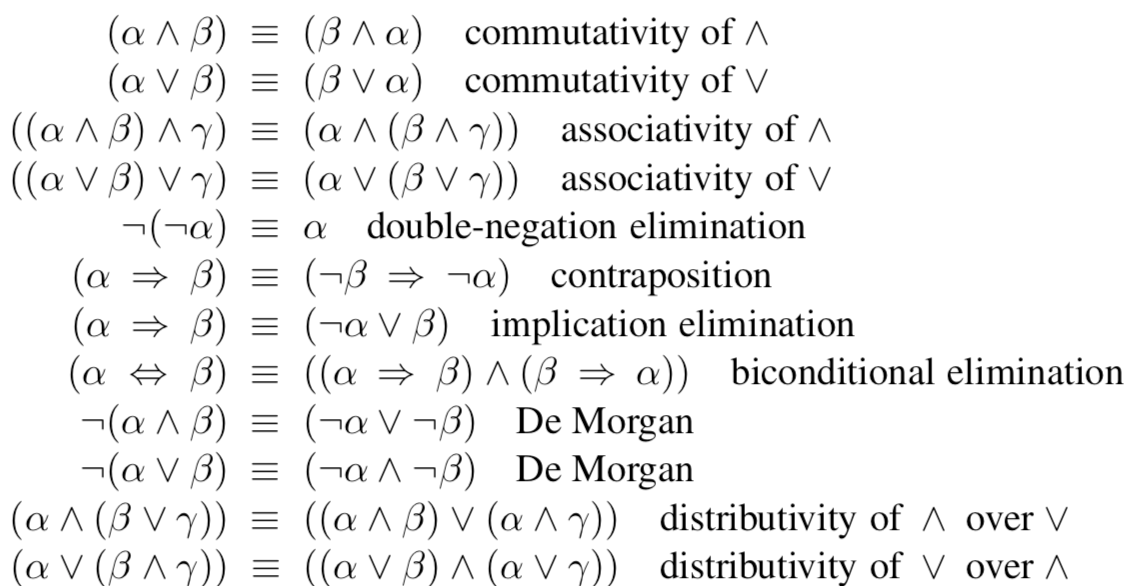
\includegraphics[width=0.9\columnwidth]{logical-equiv}
  \subsection{Resolution for Conjunctive Normal Form (CNF)}
  \begin{itemize}
    \item Conjunction of disjunction of literals
    \item if a literal $x$ appears in a clause and its negation $\lnot x$ appears in another clause, it can be deleted
    \item Resolution is \textbf{sound} and \textbf{complete} for propositional logic
    \item \textbf{Resolution thm}: if a set of clauses is unsatisfiable, then the resolution closure of those clauses contains the empty clause
  \end{itemize}
  \subsection{Forward and Backward Chaining}
  \begin{itemize}
    \item Horn clause = disjunction of literals of which at most 1 is positive
    \item Both forward and backward chaining with Horn clauses run in \textbf{linear} time
    \item Inference using \textbf{Modus Ponens}: \textbf{sound} for Horn KB
  \end{itemize}
  \subsubsection{Forward Chaining}
  \begin{itemize}
    \item Data-driven reasoning, e.g. object recognition, routine decisions.
    \item May do a lot of work irrelevant to the goal
  \end{itemize}
  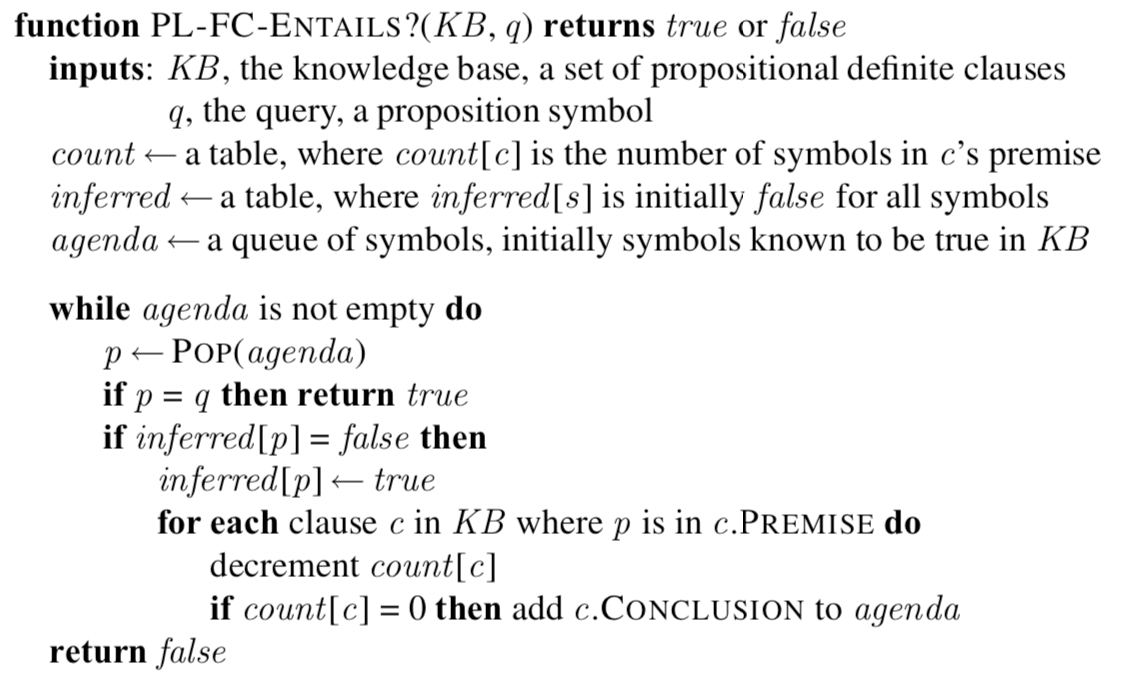
\includegraphics[width=0.9\columnwidth]{horn-fc}
  \subsubsection{Backward Chaining}
  \begin{itemize}
    \item To prove $q$ by BC, check if $q$ is known already, or prove by BC the premise of some rule concluding $q$
    \item \textbf{Avoid loops}: check if new subgoal is already on the goal stack
    \item \textbf{Avoid repeated work}: check if new subgoal already failed or proven true
    \item Goal-driven reasoning, complexity can be sublinear in size of KB
    \item Improvements over truth table enumeration:
          \begin{itemize}
            \item \textbf{Early termination}: a clause is true iff any literal in it is true; the formula is false if any clause is false.
            \item \textbf{Pure symbol heuristic} (Least constraining value): \textbf{pure symbol} always appear with the same ``sign'' in all clauses, make a pure symbol's literal true, ignore clauses already true in the model constructed so far
            \item \textbf{Unit clause heuristic}: Unic clause = only 1 literal in the clause, the only literal in a unit clause must be true.
          \end{itemize}
  \end{itemize}

  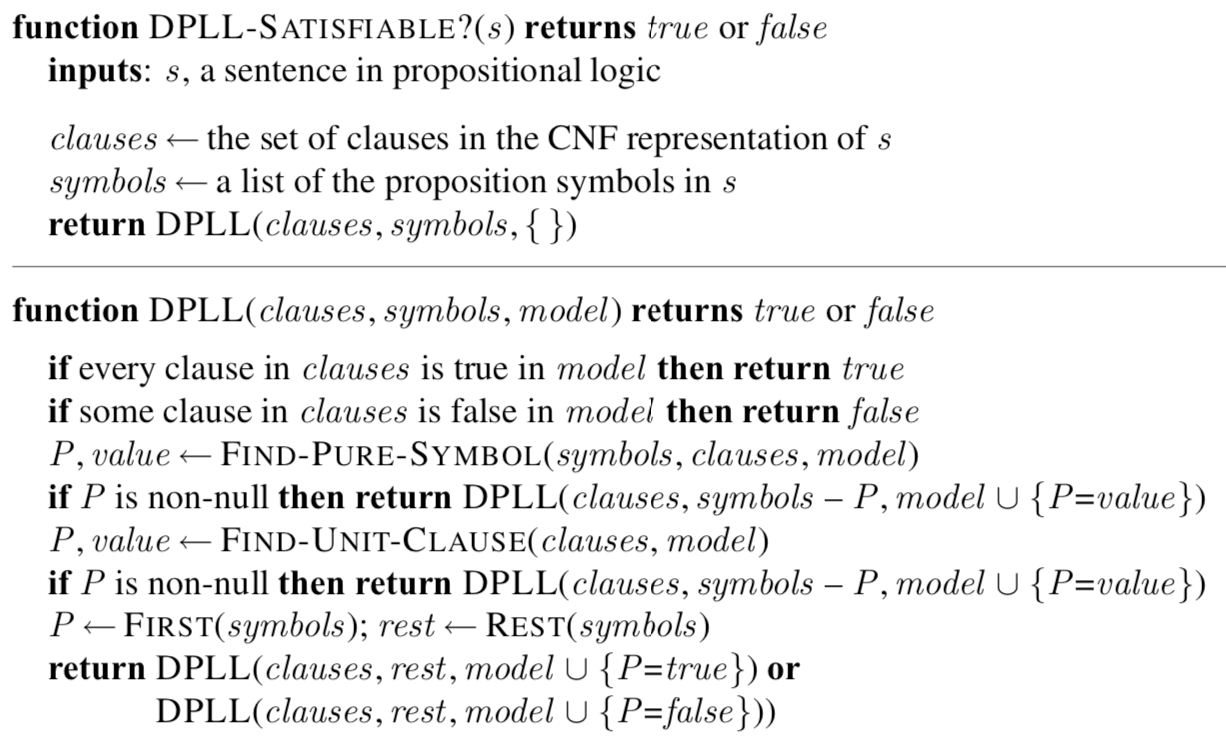
\includegraphics[width=\columnwidth]{dpll}
  \subsection{Local Search Algo: WalkSAT}
  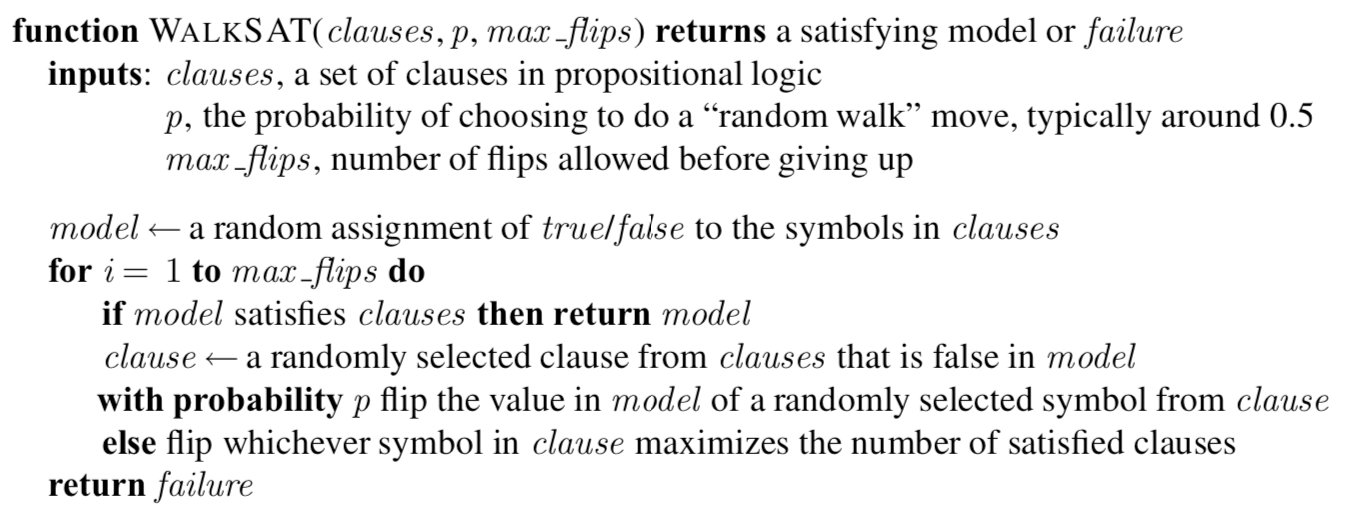
\includegraphics[width=\columnwidth]{walksat}

  \section{First-Order Logic (FOL)}
  \subsection{Syntax}
  \begin{itemize}
    \item \textbf{Constants}, e.g. John, 2, NUS
    \item \textbf{Predicates}, e.g. $Brother(x, y)$, $x > y$
    \item \textbf{Functions}, e.g. $\sqrt{x}, LeftLeg(x)$
    \item \textbf{Variables}, e.g. $x$, $y$, $a$, $b$
    \item \textbf{Operator Precedence}: $\lnot$, $=$, $\land$, $\lor$, $\implies$, $\iff$
    \item \textbf{Quantifiers}: $\forall$, $\exists$
    \item \textbf{Atomic Sentences}: constant or variable or function or predicate
    \item \textbf{Complex Sentences}: constructed from atomic sentences via connectives
  \end{itemize}
  \subsection{Semantics}
  Sentences are true in a model, comprising a set of objects (domain elements) \& an interpretation
  \subsection{Quantifiers}
  \begin{itemize}
    \item Universal ($\forall$): uses $\implies$, equivalent to conjunction of instantiations
    \item Negation of $\forall x: P(x)$ is $\exists x: \lnot P(x)$
    \item Existential ($\exists$): uses $\land$, equivalent to disjunction of instantiations
    \item Negation of $\exists x: P(x)$ is $\forall x: \lnot P(x)$
  \end{itemize}
  \subsection{Knowledge Engineering in FOL}
  (1) Identify the task,
  (2) Assemble the relevant knowledge,
  (3) Decide on a vocabulary of predicates, functions, and constants,
  (4) Encode general knowledge about the domain,
  (5) Encode a description of the specific problem instance,
  (6) Pose queries to the inference procedure and get answers,
  (7) Debug the knowledge base,

  \section{Inference in FOL}
  \subsection{Reduction to Propositional Inference}
  \begin{itemize}
    \item Every FOL KB can be propositionalised, preserves entailment: $\alpha$ is entailed by new KB iff entailed by original KB
    \item \textbf{Herbrand Thm}: If $\alpha$ if entailed by FOL KB, then it is entailed by a \textbf{finite subset} of the propositionalised KB.
    \item For $n = 0$ to $\infty$, create propositionalized $KB_n$ by instantiating with depth-$n$ terms, see if $\alpha$ is entailed by this $KB_n$, semi-decidable (return TRUE if entailed, but cannot return FALSE if not entailed)
    \item Exponential blowup: $k$-ary predicate has $n^k$ instantiation with $n$ constants, some of the things generated irrelevant
    \item Rule of \textbf{Universal Instantiation}: we can infer any sentence obtained by substituting a \textbf{ground term} (a term without variables) for the variable.
    \item Rule of \textbf{Existential Instantiation}: variable is replaced by a single new constant symbol that has not appeared elsewhere in the KB.
  \end{itemize}
  \subsection{Unification}
  \begin{itemize}
    \item Find a substitution $\theta$ such that different logical expressions look identical
    \item \textbf{Standardising apart} one of the two sentences being unified (rename to avoid name clash)
    \item There is a single unique \textbf{most general unifier} (MGU) up to renaming and substitution of variables
    \item \textbf{Occur check} to check whether the variable itself occurs inside the term, in which the match fails, e.g. $S(x)$ with $S(S(x))$ -- this makes the entire algo quadratic in the size of the expressions being unified
  \end{itemize}
  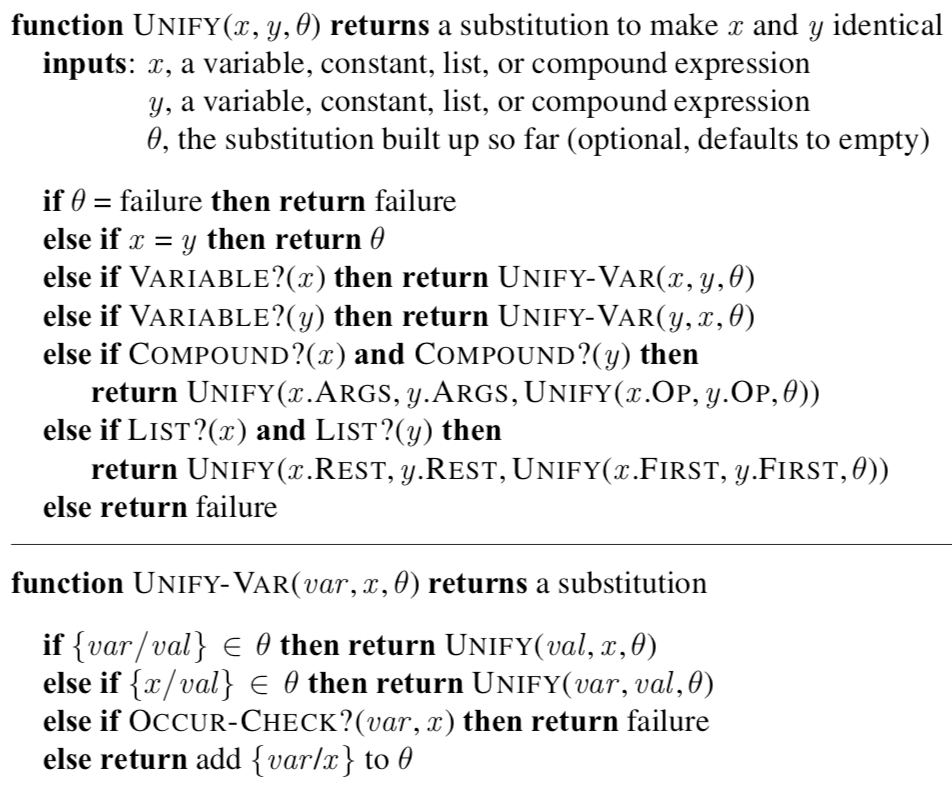
\includegraphics[width=0.8\columnwidth]{unify}
  \subsection{Generalized Modus Ponens (GMP)}
  There is some substitution $\theta$ such that the premise and the LHS of implication are the same, can infer RHS of implication
  \subsection{Forward Chaining}
  At every round, add all newly inferred atomic sentences to KB. Repeat until: one of these sentences is $\alpha$ or no new sentences can be inferred

  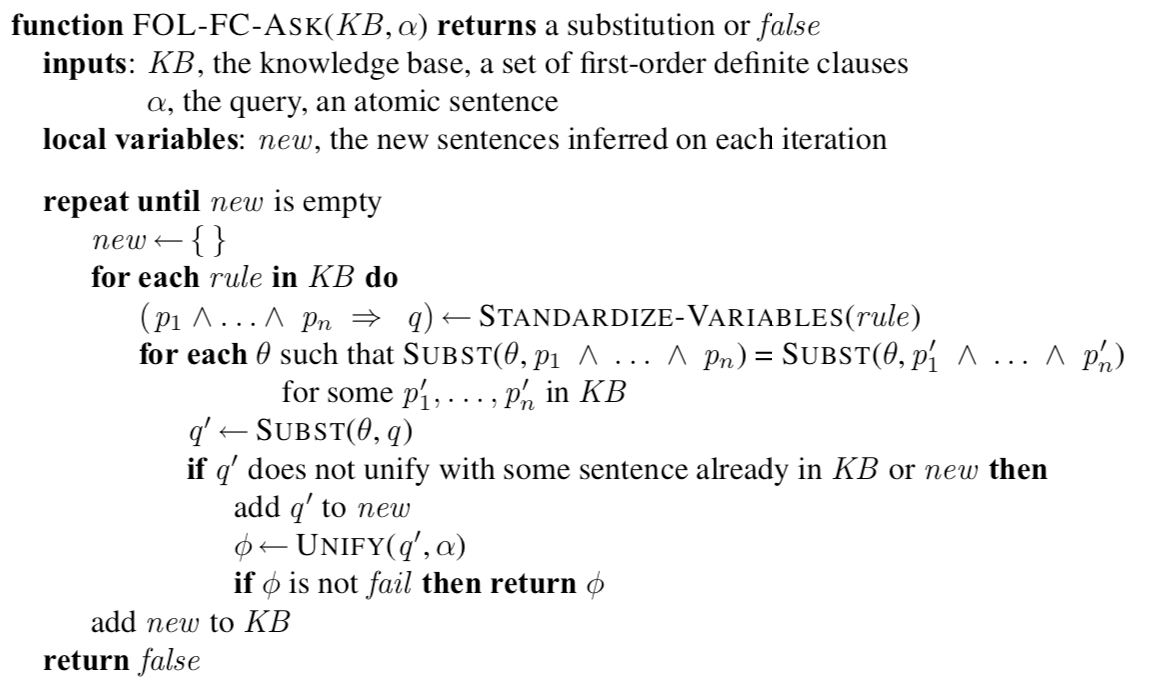
\includegraphics[width=0.9\columnwidth]{fol-fc}
  \subsubsection{Properties}
  \begin{itemize}
    \item \textbf{Sound} and \textbf{complete} for FOL definite clauses (disjunction of literals, exactly 1 is positive)
    \item Terminates in finite no of iterations if KB contains no functions
    \item May not terminate in general (with functions) if $\alpha$ is not entailed
  \end{itemize}
  \subsubsection{Inefficiencies of Foward Chaining}
  \begin{itemize}
    \item Matching rule premises to known fact (pattern matching) is costly. Solution:
          \begin{itemize}
            \item \textbf{Conjunct ordering problem}: apply minimum-remaining-values heuristic of CSP,
            \item \textbf{Predicate indexing}: constant time to retrieve known facts
          \end{itemize}
    \item Redundant rule matchings. Solution:
          \begin{itemize}
            \item \textbf{Incremental foward chaining}: match rule at time $t$ only if a conjunct in its premise unifies with new fact inferred at $t - 1$
            \item \textbf{Rete algorithm}: don't discard partially matched rules, keep track of conjuncts matched against new facts, avoid duplicate work
          \end{itemize}
    \item Generating irrelevant facts. Solution: use backward chaining
  \end{itemize}
  \subsection{Backward Chaining}
  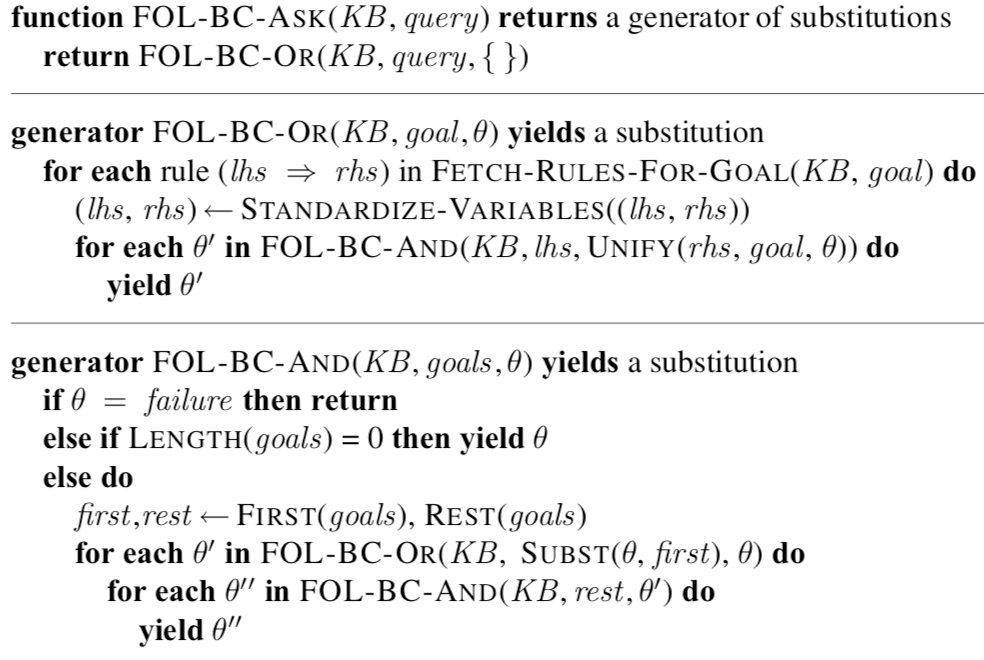
\includegraphics[width=0.9\columnwidth]{fol-bc}
  \subsubsection{Properties}
  \begin{itemize}
    \item DFS: space is linear in size of proof
    \item Incomplete due to infinite loops: fix by checking current goal against every goal on stack
    \item Inefficient due to repeated subgoals (both success and failure): fix by caching solutions to previous subgoals
  \end{itemize}

  \subsection{Resolution: convert to CNF}
  \begin{enumerate}
    \item Standardize variables,
    \item Skolemize existential quantifiers (replace with functions depending on external universal quantifier),
    \item Drop universal quantifiers,
    \item Distribute $\lor$ over $\land$
  \end{enumerate}
  \subsubsection{Resolution Inference Rule}
  \begin{itemize}
    \item FOL literals are complements if one unifes with negation of the other.
    \item First-order factoring: removes redundant literals by reducing 2 literals to one if they are unifiable (similar to propositional reducing 2 literals to one if they are identical).
    \item To prove $KB \models \alpha$, show that $KB \land \lnot \alpha$ results in contradiction
  \end{itemize}

  \subsubsection{Properties}
  Complete

  \section{Uncertainty}
  \subsection{Sources of uncertainty}
  (1) Partial observability,
  (2) Noisy sensors,
  (3) Uncertainty in action outcomes,
  (4) Complexity in modelling and predicting traffic
  \subsection{Events}
  Atomic events = an assignment of a value to each random var; a singleton event
  \subsection{Axioms of probability}
  \begin{itemize}
    \item Let $X$ be an r.v. with finite domain $D_X$
    \item A prob distribution over $D_X$ assigns a value $p_X(x) \in [0,1]$ to every $x \in D_X$ s.t. $\sum_{x\in D_X}p_X(x) = 1$
    \item $\Pr(A) + \Pr(B) = \Pr(A \cap B) + \Pr(A \cup B)$
    \item $\Pr(A \mid B) = \frac{\Pr(A \land B)}{\Pr(B)}$ assuming $\Pr(B) > 0$
    \item \textbf{Independent} if $\Pr(A \land B) = \Pr(A)$, equiv to $\Pr(A \mid B) = \Pr(A)$
    \item \textbf{Summing out}: $\Pr(X) = \sum_z\Pr(X,z)$ where $z$ is all possible value of other vars
    \item \textbf{Normalization}: in conditional, the prob of the given event is a constant $\alpha$
    \item \textbf{Bayes rule}: $\Pr(A \mid B) = \frac{\Pr(B \mid A)\Pr(A)}{\Pr(B)}$
    \item \textbf{Chain rule}: derived by successive application of Bayes rule: $\Pr(X_1 \land X_2 \land ... \land X_k) = \prod_{j=1,...,k} \Pr(X_j \mid X_1 \land ... \land X_{j-1})$
  \end{itemize}
  \subsection{Conditional Independence}
  \begin{itemize}
    \item Events are independent of each other, only related by the given event
    \item $\Pr(B \land T \mid S) = \Pr(B \mid S) \Pr(T \mid S)$
    \item Full joint distribution by chain rule: where effects are $T_i$, cause is $S$: $\Pr(T_1\land T_2\land ... \land T_n \land S) = \Pr(T_1 \mid S) \Pr(T_2 \mid S) ... \Pr(T_n \mid S) \Pr(S)$
    \item Joint distribution of $n$ boolean r.v. = $2^n - 1$ entries
    \item Conditional independence is linear
  \end{itemize}

  \section{Bayesian Networks}
  \begin{itemize}
    \item Nodes are random variables, edge from $X$ to $Y$ : $X$ directly influences Y
    \item A conditional distr for each node given its parents: $\Pr(X \mid Parents(X))$, represented as \textbf{Conditional Probability Table} (CPT): the distr of $X$ for each combination of parent values
    \item Given $X_1,...,X_n$: $\Pr(X_1 \land ... \land X_n) = \prod_i \Pr(X_i \mid Parents(X_i))$
  \end{itemize}

  \subsection{Markov Blanket}
  A node is conditionally independent of everything else given the values of its \textbf{parents}, \textbf{children}, \textbf{its children's parents}

  \subsection{d-separation}
  \begin{enumerate}
    \item \textbf{Draw the ancestral graph}: consisting of only all vars mentioned in prob expression and all their ancestors
    \item \textbf{``Moralize'' the ancestral graph by ``marrying'' the parents}: for \emph{each pair} of variables with a common child, draw an undirected edge betweeen them
    \item \textbf{``Disorient'' the graph by replacing directed edges with undirected edges}
    \item \textbf{Delete the given and their edges}
    \item \textbf{Read the answer off the graph}:
          \begin{itemize}
            \item If vars \textbf{disconnected} in graph: guaranteed to be independent
            \item If vars \textbf{connected} in graph: not guaranteed to be indep (dependent as far as Bayes net is concerned -- can still be numerically indep)
            \item If one/both of the vars missing (because they were givens), independent
          \end{itemize}
  \end{enumerate}

  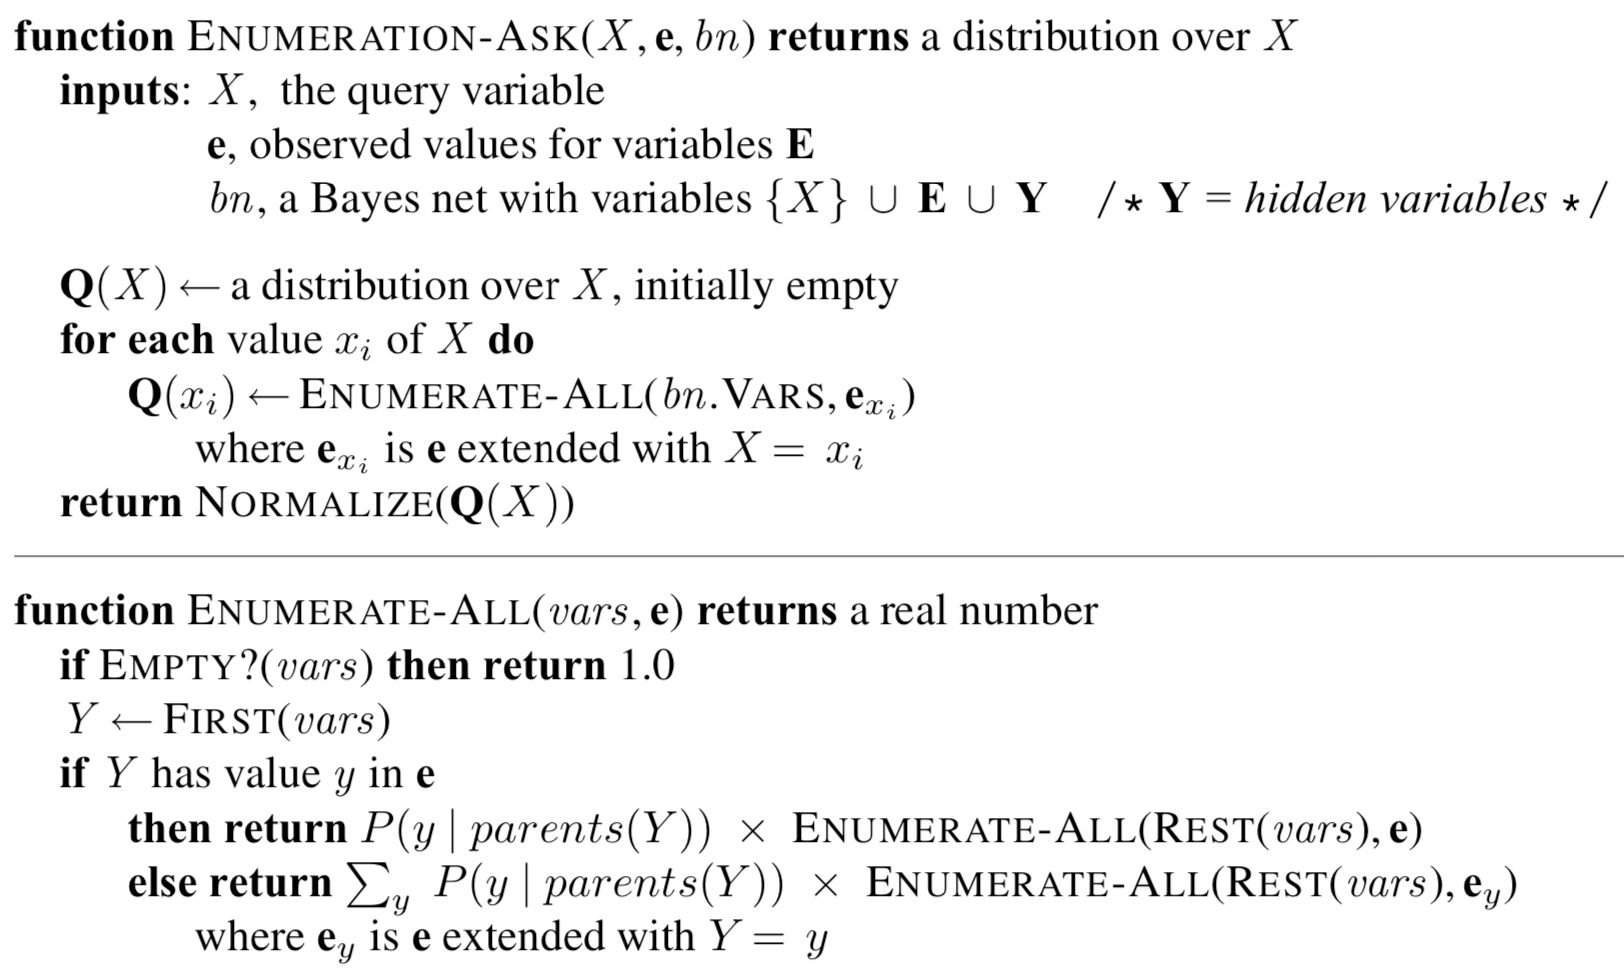
\includegraphics[width=\columnwidth]{enumeration}



\end{multicols*}
\end{document}
